\section{Discussion}
\label{s:discussion}

This section discusses the potential deployment of the system.
\subsection{Server based}

Pros:	practical, easy deployment.
cons:	IP cloaking, SEM, hard to decide crawling periods. 
Solution: IP cloaking, Buy 100k IP.
SEM, Deduce visits by search engine. 

\subsection{Crowdsource based}
Employ RAPPOR~\cite{erlingsson2014rappor} to provide user privacy gurantee.

pros: 	1.privacy 2.Low traffic. 3.SEM 4.Distributed computation 
5. Remove the need to do redirect cloaking detection, leveraging the feature
that the end goal of attackers is to reach user
6. could decide crawl period passively based on user clicks, data received are
based on real user’s clicks, say, website traffic

cons: user incentives. 
Solution: Plugin to detect suspicious websites. API


\begin{figure}[t]
  \centering
  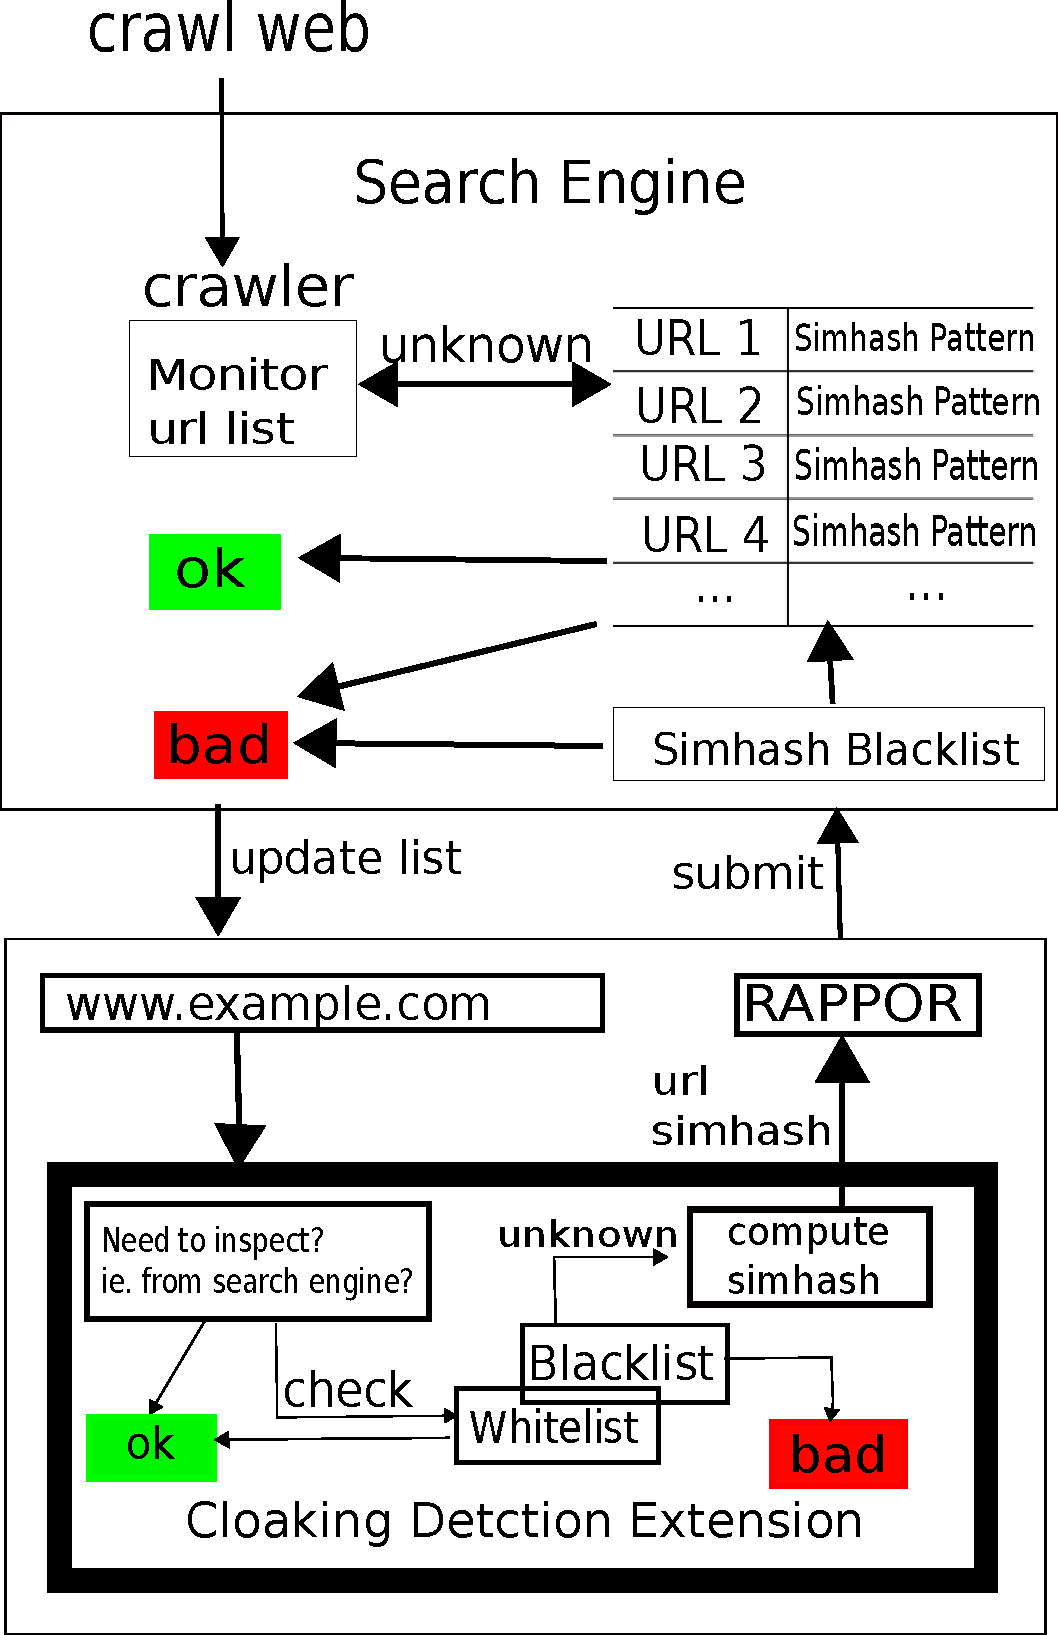
\includegraphics[width=.5\textwidth]{fig/workflow}
  \caption{Workflow of crowdsource cloaking detection sysetem}
  \label{fig:workflow}
\end{figure}


The workflow ~\autoref{fig:workflow} is to collect page contents simhash on the user side, and compare
them to simhash of the same link from ad serving company to find cloaking. When
the differences of the simhashes are significantly large, the page is marked
cloaking. We generate two simhash for page content and structure respectively.
Intuition behind this is, simhash difference between different sites are larger
than different visits of the same site. We build a two-phase system to detect
cloaking: cluster learning phase, and cloaking detection phase. In the cluster
learning phase, an ad company visit urls and generate simhash from its content
with its owned IP, and learn pattern and distribution of the simhashes, i.e.
simhash-based website model. In the cloaking detection phase, the ad company
collects simhash from its users. Compare them with learned patterns, return
cloaking score or mismatch

